\documentclass[12pt]{article}
	
%______________________PREAMBULO_________________________

%----------------------Paquetes--------------------------
\usepackage{amsmath,amssymb,amsfonts,latexsym,cancel} % Paquetes de símbolos adicionales.
\usepackage[spanish,es-tabla]{babel} % Idioma español
\usepackage[utf8]{inputenc} % Paquete que nos permite usar los acentos y otros símbolos, directamente del teclado.
\usepackage[T1]{fontenc} % Cambia el tipo de letra
\usepackage{times} % Tipo de letra Times New Roman
\usepackage{graphicx} % Paquete para el manejo de gráficos y figuras en el documento.
\usepackage{geometry} % Permite el manejo de los margenes
\usepackage{fancyhdr} % Permite colocar y manejar el encabezado
\usepackage[breaklinks,colorlinks=true,linkcolor=black,citecolor=blue, urlcolor=blue]{hyperref} % Crea hipervinculo entre secciones y el indice
\usepackage{pstricks}
\usepackage{multicol}
%\usepackage{mathpazo} %fuente palatino
%\usepackage{xcolor}
%\usepackage[shortlabels]{enumitem}
%-------------Paquetes para el formato de las citas-------
%\usepackage[hyphens]{url}
%\usepackage{float}
%\usepackage{cite}
%\usepackage{wrapfig}

%-----------------------------ayuda de paquetes--------------------

\spanishdecimal{.}

%------------------------Margenes----------------------------

\newgeometry{bottom = 2.5 cm, top = 2.5 cm, left = 2 cm, right = 2 cm} % Modifica el margen {Abajo, Arriba, Izquierda, Derecha

%----------------------------Interlineado----------------------------------

%\doublespacing
%\onehalfspace
%\singlespace
%\spacing{1.5} % Permite personalisar a gusto
%\setlength{\parskip}{2cm} % Es el espacio entre parrafos

%-----------------------------Sangria---------------------------------------

\setlength{\parindent}{0 cm} % Manipula la sangria

%---------------------Portada------------------

%\title{
%\begin{figure}[h!]
		
%	\centering
%	
\includegraphics[width=\linewidth]{Nom_UAdeC_FCFM.png}  			
			
%\end{figure}
%\huge \textbf{LABORATORIO DE FISICA 3}\\\LARGE TITULO PRACTICA\\}
%\author{ \Large \textbf{Profesor:}\\
%\Large \textbf{Alumno:} Oscar Joel Castro Contreras}
%\date{\today}

%--------------Encabezado y pie de pagina--------------------

\pagestyle{fancy}%Coloca el encabezado en el documento
\lhead[]{Métodos numéricos}%Encabezado izquierda
\rhead[]{Oscar Joel Castro Contreras}%Encabesado derecha
%\chead[]{}%Encabesado central
\renewcommand{\headrulewidth}{0.08 pt}%Coloca linea al pie de pagina

%\lfoot[]{PI}%Pie de pagina izquerdo
%\rfoot[]{PD}%Pie de pagina derecho
\cfoot[]{\thepage}%Pie de pagina central
\renewcommand{\footrulewidth}{0.08 pt}%Coloca linea al pie de pagina

%-----------------------------------------------------------------------------

	\begin{document}
		
		\begin{titlepage}
		
			\centering
			{\bfseries
			\begin{figure}[h!]
				\centering
				
\includegraphics[width=\linewidth]{Nom_UAdeC_FCFM.png} 				
			\end{figure}
			\par}
			\vspace{2cm}
			{\scshape\LARGE Métodos numéricos \par}
			\vspace{3cm}
			{\scshape\Huge \textbf{Aproximación polinomial simple e interpolación} \par}
			\vfill
			{\LARGE \textbf{Profesora:} Maria Guadalupe Godina Cubillo \par}
			\vspace{3cm}
			{\LARGE \textbf{Alumno:} Oscar Joel Castro Contreras \par}
			\vfill
			{\Large \today \par}
			\thispagestyle{empty}
			%\thispagestyle{fancy}
			
		\end{titlepage}
	
		\newpage

		\begin{abstract}
			\noindent En este reporte explico un poco lo que es la interpolación y en que consiste, también explico qué es, 
			cómo se aplica la aproximación polinomial simple a una cierta cantidad de puntos dados y cuáles son le fallos 
			que encontré al programarlo y hacer distintas pruebas con distintas series de puntos.
		\end{abstract}

		\textbf{Palabras clave:} Polinomio, interpolación, Sistema de ecuaciones.

		\section*{\centering Introducción}\label{sec:Introducción}
			Una función de interpolación es aquella que pasa a través de puntos dados como datos, los cuales 
			se muestran comúnmente por medio de una tabla de valores o se toman directamente de una función 
			dada. \\
			La interpolación de los datos puede hacerse mediante un polinomio, la interpolación polinomial 
			ajustar un polinomio a los puntos dados, es uno de los temas más importantes en métodos numéricos, 
			ya que La mayoría de los métodos numéricos se basan en la interpolación polinomial. Por ejemplo, 
			los métodos de integración numérica se obtienen integrando fórmulas de interpolación polinomial, 
			y los métodos de diferenciación numérica se obtienen derivando las interpolaciones polinomiales. \cite{bib:item1} \\
			Cuando el numero de datos disponibles es reducido para intentar obtener una ecuación o modelo 
			matemático que los represente, o simplemente se requiere una estimación rápida de un valor 
			intermedio, o fuera del intervalo de observación, resulta conveniente recurrir a la aproximación 
			polinomial. Un polinomio de enésimo orden tiene la forma siguiente:
			$$ f(x) = a_0 + a_1x + a_2x^2 + a_3x^3 + \dots + a_nx^n $$
			Y puede se ajustado a $ n+1 $ puntos, de manera que existe uno y solo un polinomio de enésimo orden 
			que pasa a través de todos los puntos. \cite{bib:item2}
		
		\section*{\centering Metodología}\label{sec:Metodologia}
			El método de aproximación polinomial simple consiste en tener nuestra tabla de puntos dados y 
			formar un polinomio de un grado enésimos dependiendo de los $ n $ datos que se tengan, este 
			polinomio cruza por todos los puntos dados.
			\begin{table}[h!]
				\centering
				\begin{tabular}{|c    c    c    c    c    c|}
					\hline
					\textbf{Puntos} & 0 & 1 & 2 & \dots & n \\\hline
					$x$ & $x_0$ & $x_1$ & $x_2$ & \dots &  $x_n$ \\\hline
					$f(x)$ & $f(x_0)$ & $f(x_1)$ & $f(x_2)$ & \dots & $f(x_n)$ \\\hline								
				\end{tabular}
				\caption{Tabulación de una función $f(x)$. \cite{bib:item3}}
				\label{tab:1}
			\end{table}
			Para poder encontrar una función polinomial con los datos de la tabla 1, primero debemos 
			crear un sistema de ecuaciones de la forma:
			\begin{align*}
				f(x_0) &= a_0 + a_1x_0 + a_2x_0^2 + \dots + a_nx_0^{n} \\
				f(x_1) &= a_0 + a_1x_1 + a_2x_1^2 + \dots + a_nx_1^{n} \\
				f(x_2) &= a_0 + a_1x_2 + a_2x_2^2 + \dots + a_nx_2^{n} \\\\
				f(x_n) &= a_0 + a_1x_n + a_2x_n^2 + \dots + a_nx_n^{n} \\
			\end{align*}
			O en forma matricial\\
			\begin{center}
				$
				\left(\begin{array}{ccccc}
					1 & x_0 & x_0^2 & \dots & x_0^{n} \\
					1 & x_1 & x_1^2 & \dots & x_1^{n} \\
					1 & x_2 & x_2^2 & \dots & x_2^{n} \\
					\vdots & \vdots & \vdots & \ddots & \vdots \\
					1 & x_n & x_n^2 & \dots & x_n^{n}
			    \end{array}\right)
			    \left(\begin{array}{c}
					a_0 \\
					a_1 \\
					a_2 \\
					\vdots \\
					a_n 
			   	\end{array}\right)
			   	=
			   	\left(\begin{array}{c}
				f(x_0) \\
				f(x_1) \\
				f(x_2) \\
				\vdots \\
				f(x_n) 
		   		\end{array}\right)
			   	$
			\end{center}
			Al resolver este sistema por el método que más conveniente, obtendremos el valor de $ a_0 $, $ a_1 $, $ a_2 $, hasta $ a_n $ y podremos 
			construir el polinomio de la forma:
			$$ P(x) = a_0 + a_1x + a_2x^2 + \dots + a_nx^{n} $$
			Este polinomio $ P(x) $ al graficarlo o evaluarlo pasara por los puntos dados de la tabla \ref{tab:1}.

		\section*{\centering Resultado}\label{sec:Resultado}
			\begin{table}[h!]
				\centering
				\begin{tabular}{|c    c    c    c    c    c    c    c|}
					\hline
					\textbf{Puntos} & 0 & 1 & 2 & 3 & 4 & 5 & 6 \\\hline
					\textbf{T($^0C$)} & 56.5 & 78.6 & 113.0 & 144.0 & 181.0 & 205.0 & 214.5 \\\hline
					\textbf{P(atm)} & 1 & 2 & 5 & 10 & 20 & 30 & 40 \\\hline								
				\end{tabular}
				\caption{Temperatura de ebullición de la acetona a diferentes presiones, datos completos. \cite{bib:item3}}
				\label{tab:2}
			\end{table}
			\begin{table}[h!]
				\centering
				\begin{tabular}{|c    c    c    c|}
					\hline
					\textbf{Puntos} & 0 & 1 & 2 \\\hline
					\textbf{T($^0C$)} & 56.5 & 113.0 & 181.0 \\\hline
					\textbf{P(atm)} & 1 & 5 & 20 \\\hline								
				\end{tabular}
				\caption{Temperatura de ebullición de la acetona a diferentes presiones, datos incompletos. \cite{bib:item3}}
				\label{tab:3}
			\end{table}
			Tenemos estas tablas de datos, la tabla \ref{tab:2} tiene mas datos que la tabla \ref{tab:3}. En la tabla \ref{tab:3} se redujo 
			el numero de datos para poder hacer él polinomio más fácilmente que usando todos los datos de la 
			tabla \ref{tab:2}. Con el polinomio obtenido de los datos de la tabla \ref{tab:3} podremos aproximarnos a los 
			valores de la tabla \ref{tab:2} que no están en la tabla \ref{tab:3}.
			Siguiendo la explicación de antes tomamos los puntos de la tabla \ref{tab:3}, para crear nuestro sistema de ecuaciones y obteniendo:
			\begin{align*}
				56.5 &= a_0 + a_1(1) + a_2(1)^2 \\
				113 &= a_0 + a_1(5) + a_2(5)^2 \\
				181 &= a_0 + a_1(20) + a_2(20)^2 
			\end{align*}
			\begin{center}
				$
				\left(\begin{array}{ccc}
					1 & 1 & 1 \\
					1 & 5 & 25 \\
					1 & 20 & 400 \\
			    \end{array}\right)
			    \left(\begin{array}{c}
					a_0 \\
					a_1 \\
					a_2 
			   	\end{array}\right)
			   	=
			   	\left(\begin{array}{c}
				 56.5 \\
				 113 \\
				 181 
		   		\end{array}\right)
			   	$
			\end{center}
			Al resolver el sistema llagamos a que, $ a_0 = 39.85 $, $ a_1 = 17.15$, y $ a_2 = -0.5048 $.
			Solo falta acomodar estos valores de la forma antes explicada para crear el polinomio $ P(x) $ 
			de los puntos de la tabla \ref{tab:3}, el polinomio es:
			$$ P(x) = -0.5048x^2 + 17.15x + 39.85 $$
			Ahora hay que evaluar esta función en los datos de la tabla \ref{tab:2} que no están en la tabla \ref{tab:3} una y 
			obtendremos una aproximación de estos valores que se muestran en la tabla \ref{tab:4}. 
			\begin{table}[h!]
				\centering
				\begin{tabular}{|c    c    c    c    c|}
					\hline
					\textbf{Puntos} & 0 & 1 & 2 & 3 \\\hline
					\textbf{T($^0C$)} & 72.1 & 161 & 100.1 & -81.7 \\\hline
					\textbf{P(atm)} & 2 & 10 & 30 & 40 \\\hline								
				\end{tabular}
				\caption{Datos aproximado de la tabla \ref{tab:2} con la función $P(x)$ obtenida con los datos de la tabla \ref{tab:3}.}
				\label{tab:4}
			\end{table}
			Si observamos los datos de la tabla \ref{tab:4}, si se aproximan a los de la tabla \ref{tab:2}, estas aproximaciones se 
			pueden ver mejores si se usan mas datos de los que se usaron en la tabla \ref{tab:3}, pero esto conlleva a 
			tener que resolver un sistema de ecuaciones aun mas grande y obtener una función polinomial de grado 
			aun mayor, por esta razón es mejor crear un programa que realice todo. 
			Realizando todo el procedimiento anterior con mi programa obtengo:
			\begin{center}
				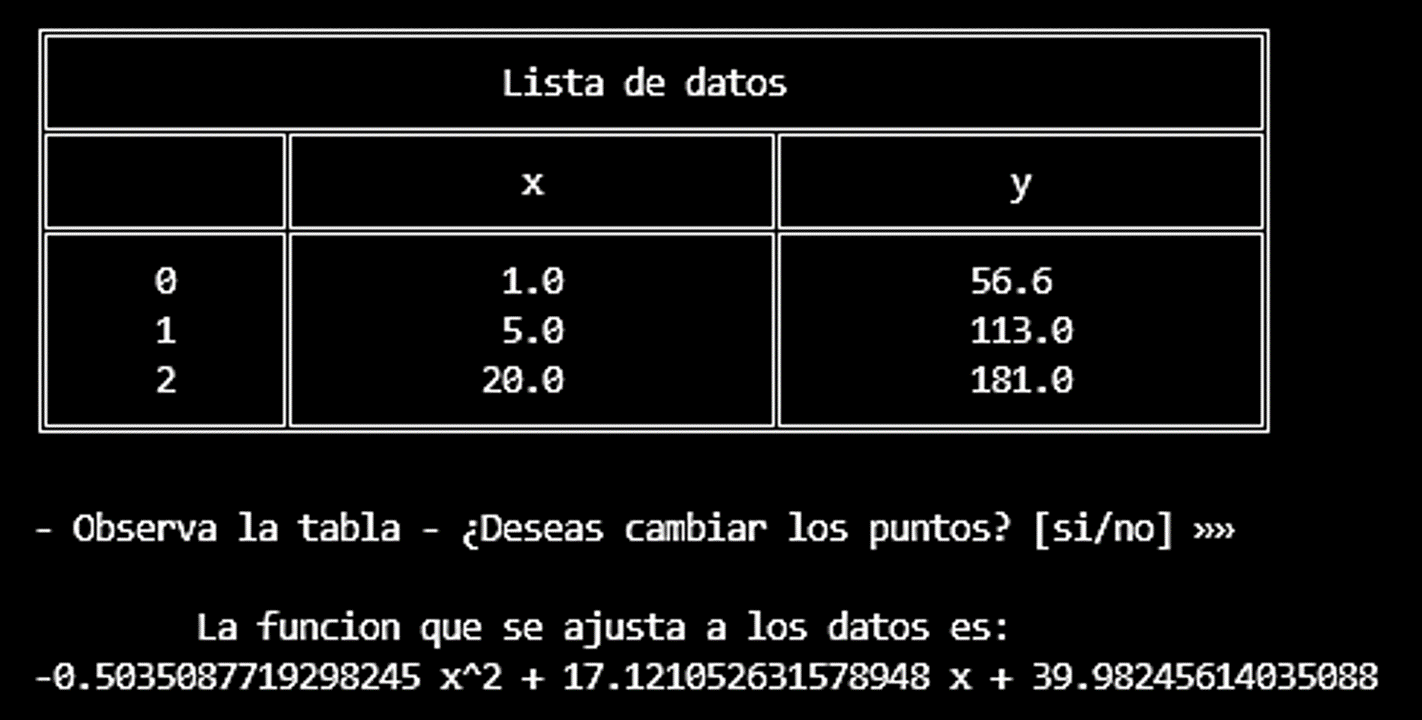
\includegraphics[width=\linewidth]{Figura 1.png}
				Figura 1: Función creada por mi programa a partir de los datos de la tabla \ref{tab:3}
				\label{Fig:1}
			\end{center}
			Se puede ver que la ecuación es la misma, solo que tiene todos los decimales que puede usar la computadora, mi programa 
			también grafico los datos y la función como se puede ver en la gráfica 1:
			\begin{center}
				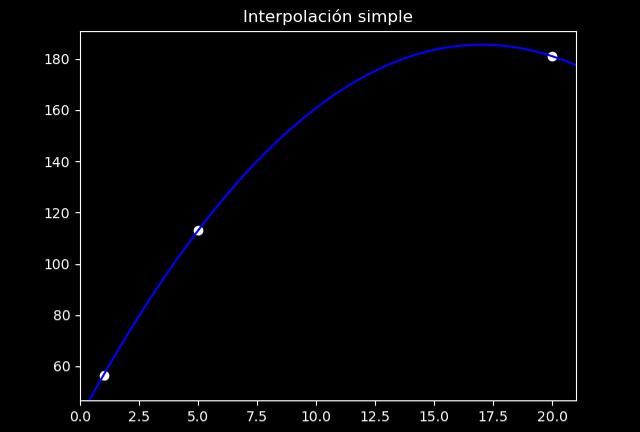
\includegraphics[width=.9\linewidth]{Grafica 1.png}\\
				Grafica 1: Grafica de la función $ P(x) $ obtenida de los datos de la tabla \ref{tab:3}
			\end{center}
			En la grafica 1 se puede observar que la función si cruza por los datos de la tabla \ref{tab:3}, ahora realizare 
			lo mismo, pero con todos los datos de la tabla \ref{tab:2}.
			\begin{center}
				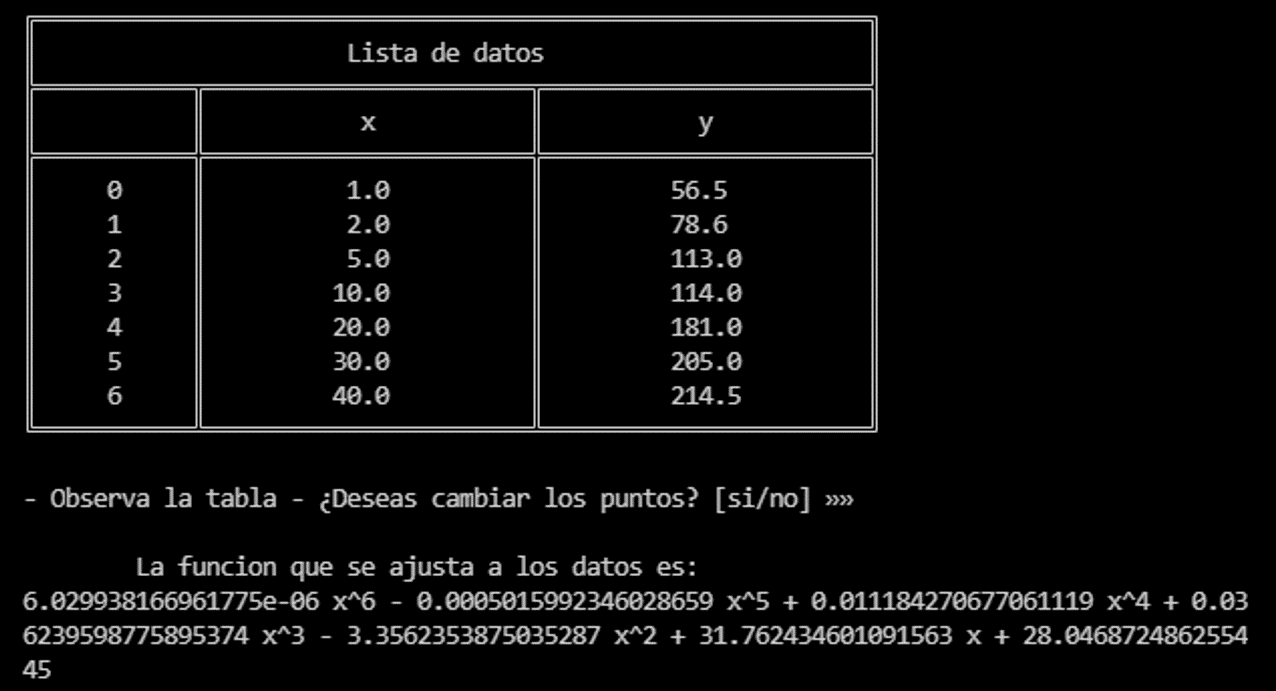
\includegraphics[width=\linewidth]{Figura 2.png}
				Figura 2: Función creada por mi programa a partir de los datos de la tabla \ref{tab:2}
				\label{Fig:2} 			
			\end{center}
			Si vemos la función es de grado 6, si le reducimos las cifras significativas podemos ver mejor la función:
			$$ 6.03 \times 10^{-6} x^6 - 5.01 \times 10^{-4} x^5 + 1.12 \times 10^{-2} x^4 + 0.036 x^3 - 3.36 x^2 + 31.8 x + 28.0 $$
			Ahora si graficamos los datos de la tabla \ref{tab:2} y la función que me da mi programa, mi programa arroga la gráfica 2.
			\begin{center}
				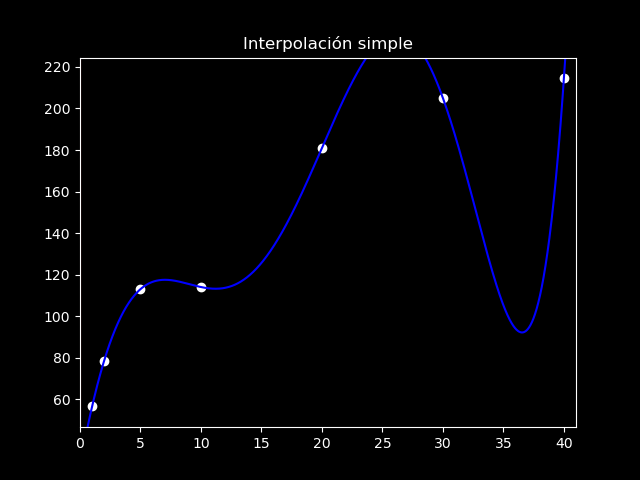
\includegraphics[width=.9\linewidth]{Grafica 2.png}\\
				Grafica 2: Grafica de la función obtenida de los datos de la tabla \ref{tab:2}
			\end{center}
		\section*{\centering Observación}\label{sec:Observacion}
			Al hacer pruebas con mi programa de distintas tablas de datos, casi en toda podía se podía ajustar 
			una función, pero en algunas no se podía, lo que tenían en común es que además de ser muchos datos, 
			los valores que había en x se repetían mucho, por ejemplo, había más de cinco $ x = 1 $ o $ x = 3 $ 
			y de igual forma con los valora en $ y $. En estos casos la función obtenida a veces solo cruzaba 
			por uno de estos puntos que se repetía y en otras ocasiones no cruzaba por ningunos.\\
			Cuando los puntos están muy dispersos y son muchos este método no es el mejor para obtener 
			una aproximación de los datos que no se conocen de la lista de datos, ya que cuando esto 
			ocurre la función solo cruza por lo puntos pero no sigue una trayectoria uniforme sino que varia mucho 
			dependiendo de la posición en la que estén, por ejemplo, si observamos la gráfica 1, esta forma 
			una curva uniforme, no varia mucho, pero si observamos la grafica 2, donde se usan mas puntos, 
			la grafica varia mucho en el espacio que hay entre cada punto, por esta razón este método no 
			es el mejor para obtener las aproximaciones.

		\section*{\centering Conclusión}\label{sec:Conclusion}
			El método toma los puntos o datos dados en una tabla, con este punto se crea un sistema 
			de ecuaciones para obtener los coeficientes de la función que cruzará por todos los puntos, 
			dependiendo de cuantos puntos sean, el polinomio sera de un grado mayor mientras mas puntos 
			se tengan y de grado menor mientras menos puntos se tengan, al resolver el sistema de ecuaciones, 
			que siempre tendrá solución ya que, si colocamos el sistema en forma matricial, podemos ver que 
			la primera fila es de puros unos. Con los resultados del sistema, los acomodamos de forma que se 
			cree la función polinomial y esta tenga un grado igual al numero de puntos usados, esta función 
			cruzara todos los puntos usados.

		\centering
		\begin{thebibliography}{10}
			\bibitem{bib:item1} Nakamura, S. (1998). Metodos Numericos Aplicados Con Software. En Solución de ecuaciones no lineales (Primera ed., pp. 62–63). Prentice Hall.
			\bibitem{bib:item2} Federico, D. S. C., \& Antonio, N. H. (2014). Métodos Numéricos Aplicados a la Ingeniería. En Método de Müller (Primera ed., pp. 79–85). Grupo Editorial Patria.
			\bibitem{bib:item3} Federico, D. S. C., \& Antonio, N. H. (2014). Métodos Numéricos Aplicados a la Ingeniería. En Aproximación funcional e interpolación (Primera ed., pp. 370–373). Grupo Editorial Patria.
		\end{thebibliography}

	\end{document}